\documentclass[12pt,a4paper]{article}
\usepackage[pdftex]{graphicx}
\usepackage{float}
\usepackage{listings}


\begin{document}
\author{
	Maciej Najdecki, s12563\\
	Krystian Rygiel, s12809\\
	Krzysztof Nowicki, s12824
}
\title{
	Human Activity Recognition\\
	using Smart Phones
}
\maketitle
\newpage

\tableofcontents
\newpage

\section{Task description}
This report covers the classification of experiment results which was performed on group of 30 volunteers. Each person performed six activities (WALKING, WALKING{\_}UPSTAIRS, WALKING{\_}DOWNSTAIRS, SITTING, STANDING, LAYING) wearing a smartphone (Samsung Galaxy S II) on the waist. Using its embedded accelerometer and gyroscope, 3-axial linear acceleration and 3-axial angular velocity at a constant rate of 50Hz were captured. The experiments have been video-recorded to label the data manually.\\
The main purpose of this project is to perform \textbf{feature selection} and \textbf{classification} of the feature vectors. The experimental process of developing program and performing experiment has been widely described in further sections of this article.

\section{Initial dataset}
The dataset has been downloaded from the \textbf{UCI} repository from link assigned to this particular problem, the \textbf{Human Activity Recognition using Smart Phones}. The brief description of the data may be found there.\\
Due to task requirements, we were supposed to train classifier on the entire dataset. The datasource was already splitted as two distinct non overlapping sets-  training and testing one. Task requires to split entire set randomly, so first of all we have merged sets to the one containing all training and testing instances.\\
\subsection{Number of records}
After successful merging of training and testing instances to single datasource it contains \textbf{10299} instances in total. Due to dataset characteristics they reside as two separate files, one with feature vectors  (\textit{dataset/train{\_}features.txt}) and second one with decision class indexes (\textit{dataset/train{\_}labels.txt}).
\subsection{Number of attributes}
Each instances is described by feature vector with length equal to \textbf{561}. The description of each feature meaning can be found on UCI webpage. Names and indexes of all features may be found in file (\textit{dataset/features.txt}).
\subsection{Decision classes distribution}
The decision class of instance is one from the predefined set \{WALKING, WALKING{\_}UPSTAIRS, WALKING{\_}DOWNSTAIRS, SITTING, STANDING, LAYING\}.\\
There are \textbf{6} decision classes assigned to the instances. The labels are stored in 4th data file called (\textit{dataset/activity{\_}labels.txt})
\subsection{Preprocessing}
Task is highly related with attributes filtering. We decided to use \textbf{WEKA} machine learning library to preprocess (filter out) redundant features. The library accepts only files with .arff format, so we wrote a converter in \textbf{Python 3.4} to create such file. The script (\textit{scripts/arff{\_}maker.py}) is responsible to merge four mentioned data files in to the single .arff one which could be further processed by WEKA library.\\
To perform the file concatenation following command must be run in shell terminal (assuming that current pwd is script folder). It is vital to redirect the output of the script to file with .arff extension, like:\\
\begin{lstlisting}[language=bash]
  ./arff_maker.py \
    ../data/features.txt \
    ../data/activity_labels.txt \
    ../data/train_features.txt \
    ../data/train_labels.txt > ../datasets/dataset.arff
\end{lstlisting}

Above command will join files together and make the valid .arff datasource file which may be used as input to weka.jar to filter attributes.

\section{Solving method}
There were to possible approaches to solve the chosen task. The \textbf{K-nearest neighbours} alogrithm and \textbf{multilayer neural network} implementation. We have decided not to use ready to go classifiers from WEKA package but we developed our implementation of multilayer network which is learned by applying backpropagation algorithm. Due to fact that all of us are familiar with \textbf{Java} programming language we have decided to implement the solving algorithm in this environment. We developed a program solution that is fully configurable via command line arguments. All of \textbf{neural network} parameters 
\subsection{Dataset filtering}
After executing command to merge data files the .arff datasource was produced so we were able to load it to the WEKA library (\textit{version 3-8-0}). It takes a while because the file is quite large (over 88MB).\\
\begin{figure}[H]
\centering
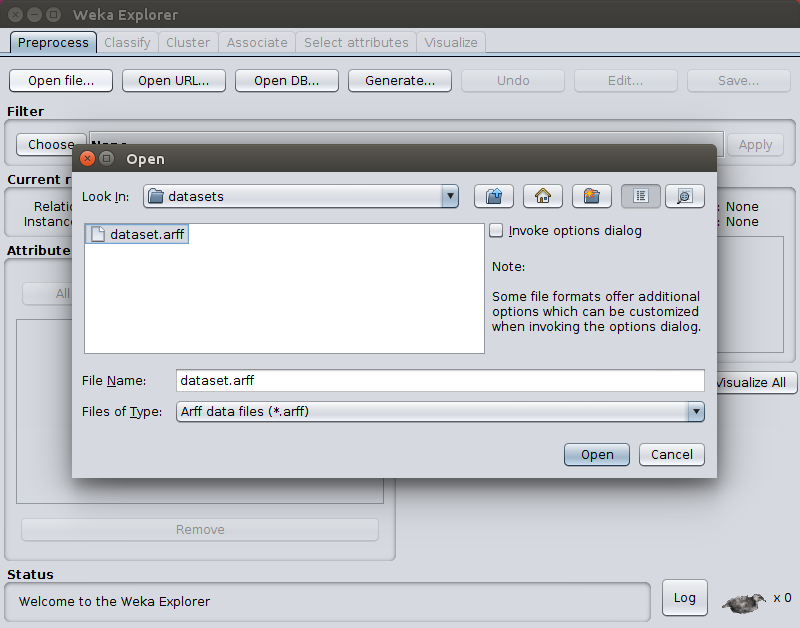
\includegraphics[scale=0.3]{img/Weka1.png}
\caption{Data loading to WEKA library}
\end{figure}

The file loads up with success so we can start adjust attribute selection options.
\begin{figure}[H]
\centering
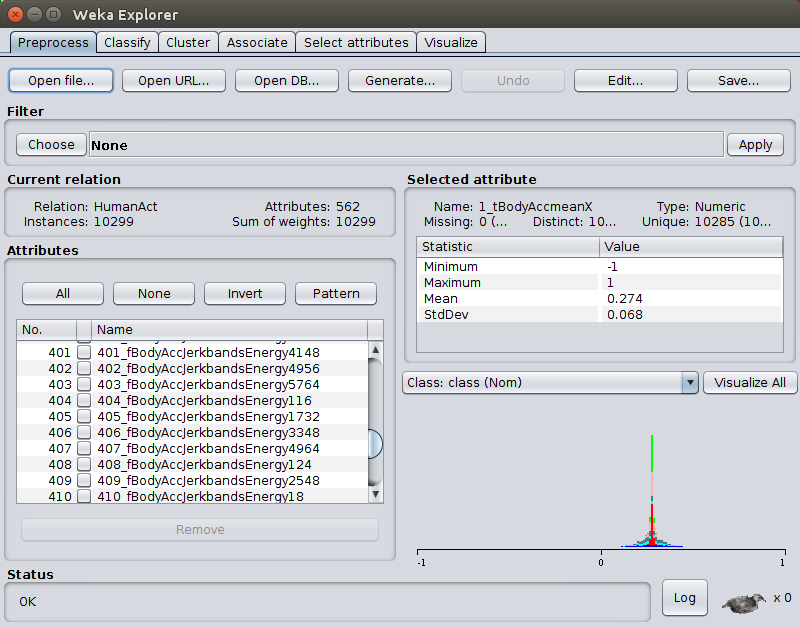
\includegraphics[scale=0.3]{img/Weka2.png}
\caption{Successfull load of data to WEKA}
\end{figure}
\subsection{Feature selection}
As a an attribute evaluator algorithm to select most vital features we used \textbf{InfoGainAttributeEval} which allows to evaluate the worth of an attribute by measuring the information gain with respect to the class. The algorithm requires \textbf{Ranker} search method to rank the attributes by their individual evaluations.\\
We performed several feature selections but finally we agreed to carry out experiment in the \textbf{4} data sets. The first one without \textbf{any attributes removed}, second with \textbf{50} most valuable attributes, third one with \textbf{20} attributes and finally the last dataset trimmed down to only \textbf{8} features from starting \textbf{561} ones. \\
\begin{figure}[H]
\centering
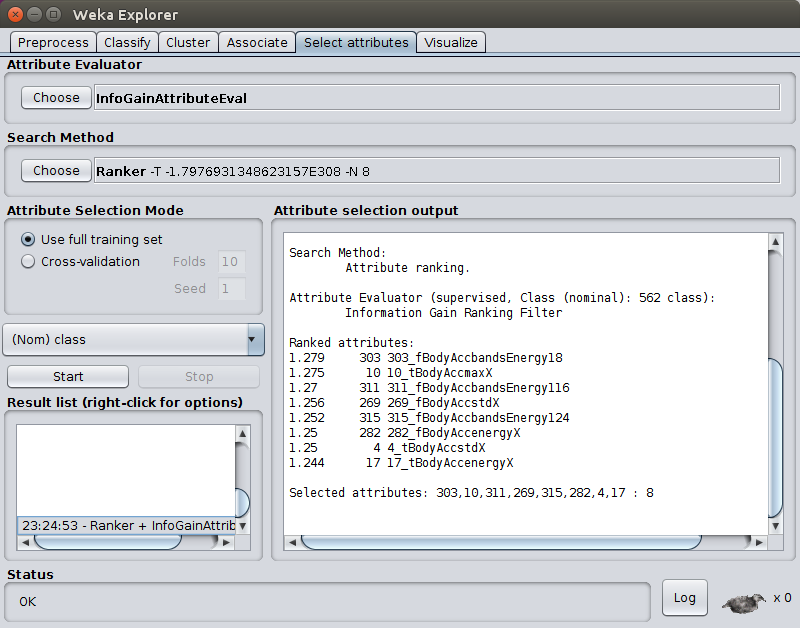
\includegraphics[scale=0.3]{img/Weka3.png}
\caption{Reducing dataset to 8 features}
\end{figure}
All information related to feature reduction operations have been saved to the \textit{filtering/} folder with appropriate names.

\section{Classification algorithm}
As previously said, we have implemented the neural network in the Java program. The final code is fully configurable via CLI arguments. There is no need to edit and recompile the program in order to check different neural network structure.
\subsection{Implementation}
The solution mainly bases on learning neural network using backpropagation algorithm. Wide spectrum of control parameters can be used to test and evaluate implemented architecture of feed forward net.\\
Implemented dynamic neural network is build with neurons which use the \textbf{SigmoidUnipolar} activation function. The used encoding for decision classes is the \textbf{Class Per Neuron} approach. The net has always fixed numbers of output layer neurons basing on passed training set.\\
Our solution is applicable to all .arff data source files, because we decided to disable configuration of last layer and provided the neuron creation for first layer neurons basing on the feature vector size.\\
Created neurons have their weights randomized by default. The range of initial synaptic weights values comes from $<-1;1>$ range.\\
What is more, our solution allows to randomly split loaded dataset to two distinct sets. The training and testing one. \\
User is able to select up to 6 different parameters, like:
\begin{lstlisting}[language=bash]
 -a <arg>   alpha parameter value (double)
 -e <arg>   number of epochs (double)
 -f <arg>   dataset arff file path (string)
 -l <arg>   hidden layers size, eg. "16,16,8" (string)
 -n <arg>   learning step value (double)
 -r <arg>   dataset instances ratio (double)
\end{lstlisting}

To perform the classification proces of given data, the program must be run with all above parameters, the example command is placed below:
\begin{lstlisting}[language=bash]
java -jar human-act-recognition.jar \
   -a 1.0 \
   -e 250 \
   -f datasets/50.arff \
   -l 16,16,8,8 \
   -n 0.01 \
   -r 0.8 > results.csv
\end{lstlisting}

The command will run progran and force it to load the dataset with \textbf{50} features. Dataset will be converted to \textbf{training} and \textbf{testing} dataset with \textbf{0.7} ratio. Initial neural net will have \textbf{4} hidden layers with \textbf{16}, \textbf{16}, \textbf{8}, \textbf{8} neurons respectively and \textbf{6} neurons in output layer, because dataset has 6 labels in total. Overall number of layers is \textbf{5}. Given alpha parameter value will be set to \textbf{1.0} and weights during learning process will be corrected with \textbf{0.01} learning step factor. Statistics of the runtime will be stored in \textit{\textbf{results.csv}} file.


\subsection{Evaluation}
During runtime of the program, it prints out 3 statistics related to learning process (\textbf{epoch}, \textbf{mean squared error}, \textbf{accuracy}). We decided to use mean squared error and accuracy as main factors that describe the neural net learning cycle. The mean squared error and accuracy can tell us, how good is the neural net performance and allows to perform simple evaluations basing on network structure, alpha parameter, weight correction step. As an accuracy we treat number of correctly classified instances over total number of instances from training set. Below statistics are already being printed in .csv format.
\begin{lstlisting}[language=bash]
0;1.5334804371559438;0.17815533980582524
1;0.8314198748395322;0.1912621359223301
2;0.830396988314016;0.1912621359223301
3;0.8280940005113736;0.20242718446601943
4;0.8230371696158392;0.1912621359223301
5;0.809863349030018;0.1912621359223301
6;0.7697027261498046;0.34563106796116505
7;0.7091877585204011;0.3257281553398058
.......
...
\end{lstlisting}

\subsection{Learning statistics}
The raw numbers representing MSE and accuracy can be easily converted to plots by executing simple script which takes the data in .csv format and prints a charts from it. Two chart makers were implemented, one for MSE, second for accuracy. In order to run data converting below shell command must be run (assuming its typed from scripts folder):\\
\begin{lstlisting}[language=bash]
./plot_mse_maker.py ../results.csv results_mse
./plot_accuracy_maker.py ../results.csv results_accuracy
\end{lstlisting}

Following command will convert the .csv records to the plots. The charts are used in next section describing experiment.


\section{Experiment}
Before the major core experiment, a lot of minor experiments were performed. It allowed us to determine the values of the configuration properties to carry out final evaluation performed on the datasets with different amount of attributes.\\
The main purpose of this task is to determine the influence of number of attributes to the classification accuracy so we assumed that the most vital part is to describe the differences between each datasets.\\
During the experiental phase we faced the problem related to too high value of learning step parameter. The accuracy was unstable, because the network was correcting its weights too fast. It happen, that it probably forgets the vectors classified correctly.\\
Too simple architecture was also a problem, because the net could not be trained on only few neurons due to too many features available. The noise which was present in the features blocked the ability to learn the simple net.
\subsection{Parameters}
Below runtime and network parameters were used to perform first experiment:\\
\begin{lstlisting}[language=bash]
Hidden layers size: 32,16,8 - overall 3 hidden layers
Output layer size:  6       - decision classes 
Alpha parameter:    1.0     - standard factor
Learning step:      0.015   - prevents fitting to data
Set ratio:          0.7     - from excercise assumptions
Epochs:             200     - enough to make conclusion
\end{lstlisting}

Additionally, we assumed that performing such experiment on only one network configuration is not enough. Below are parameters used for second analysis. The network is not as complex as previously.

\begin{lstlisting}[language=bash]
Hidden layers size: 6,6     - overall 2 hidden layers
Output layer size:  6       - decision classes 
Alpha parameter:    1.0     - standard factor
Learning step:      0.1     - will cause faster learning
Set ratio:          0.7     - from excercise assumptions
Epochs:             200     - same as before
\end{lstlisting}

\subsection{8 features}
\subsubsection{1st configuration}
\begin{figure}[H]
\centering
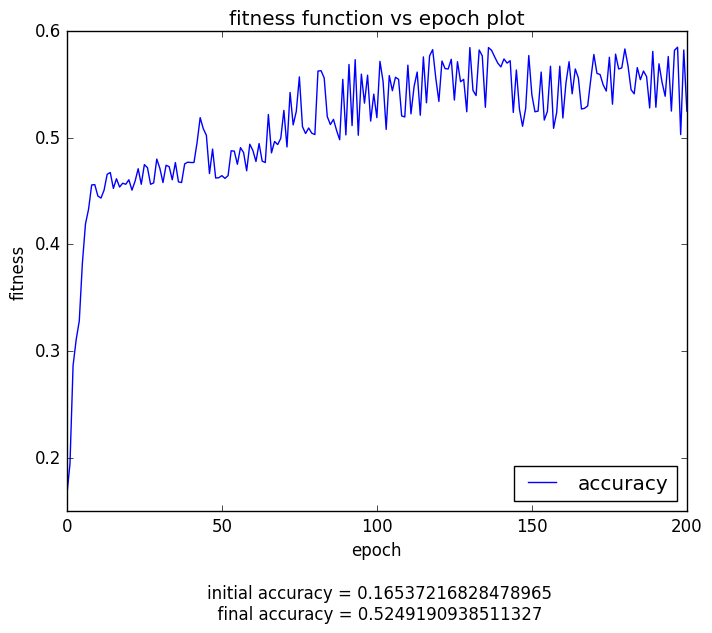
\includegraphics[scale=0.4]{img/8_acc.png}
\caption{Accuracy plot}
\end{figure}
\begin{figure}[H]
\centering
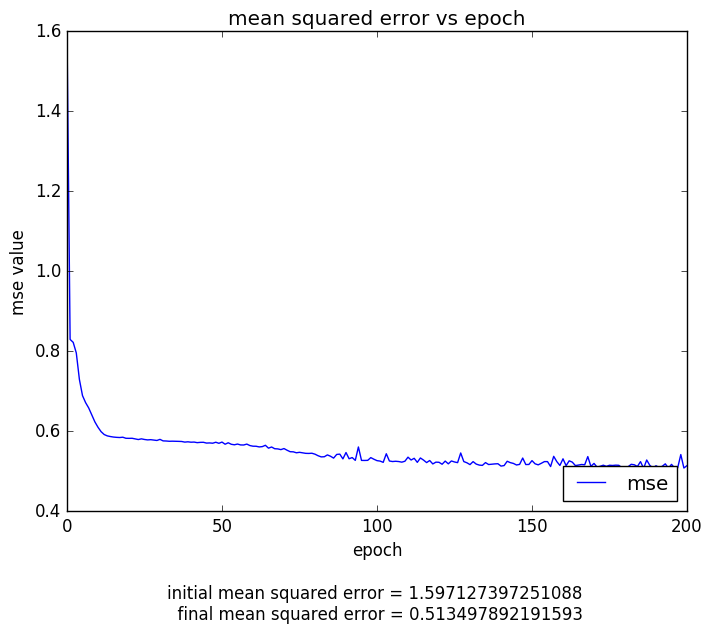
\includegraphics[scale=0.4]{img/8_mse.png}
\caption{MeanSquaredError plot}
\end{figure}

\subsubsection{2nd configuration}
\begin{figure}[H]
\centering
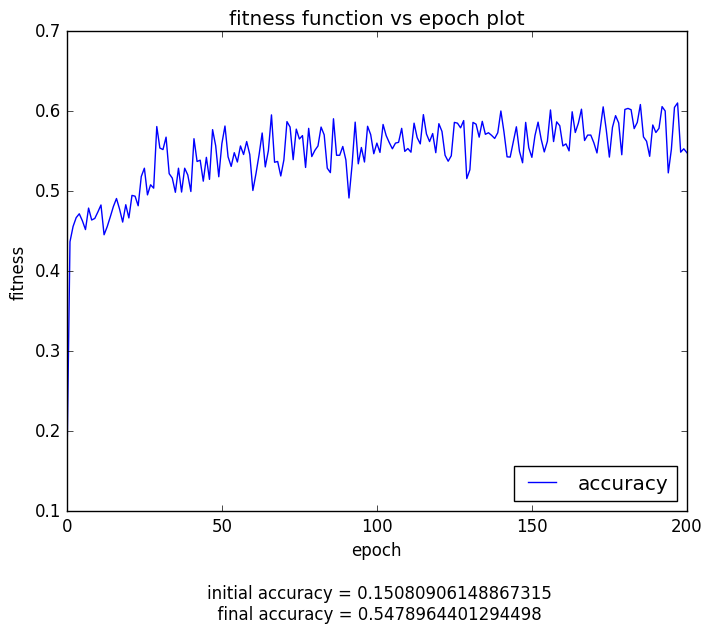
\includegraphics[scale=0.4]{img/8_acc_2.png}
\caption{Accuracy plot}
\end{figure}
\begin{figure}[H]
\centering
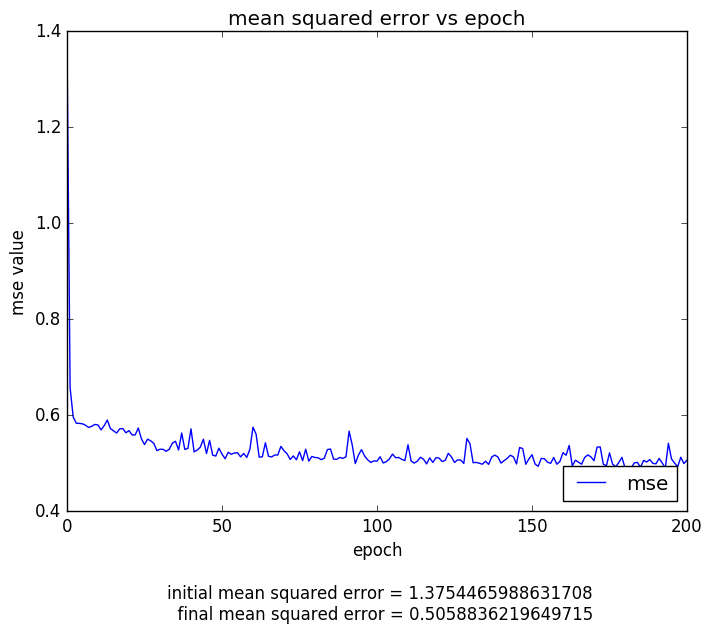
\includegraphics[scale=0.4]{img/8_mse_2.png}
\caption{MeanSquaredError plot}
\end{figure}

\subsection{20 features}
\subsubsection{1st configuration}
\begin{figure}[H]
\centering
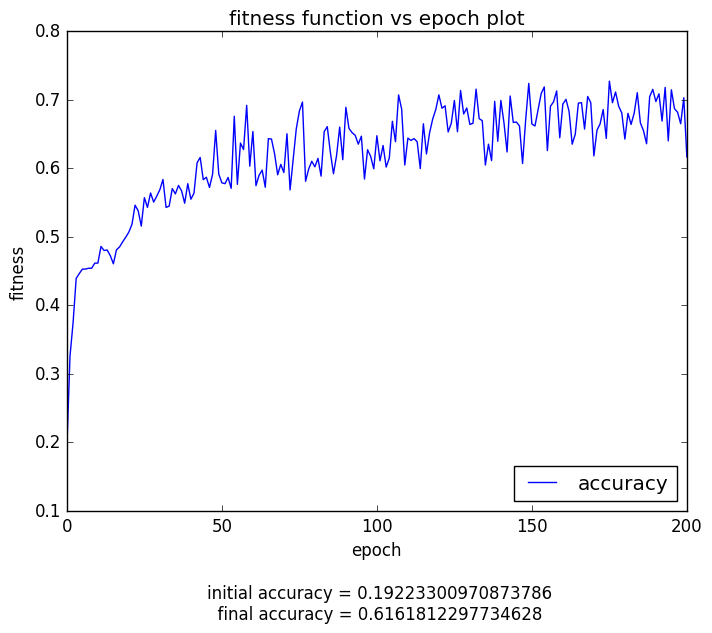
\includegraphics[scale=0.4]{img/20_acc.png}
\caption{Accuracy plot}
\end{figure}
\begin{figure}[H]
\centering
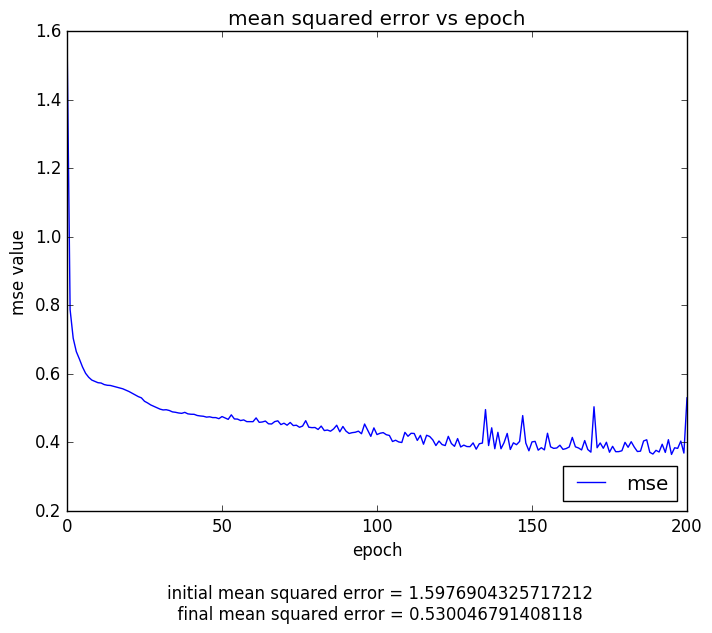
\includegraphics[scale=0.4]{img/20_mse.png}
\caption{MeanSquaredError plot}
\end{figure}

\subsubsection{2nd configuration}
\begin{figure}[H]
\centering
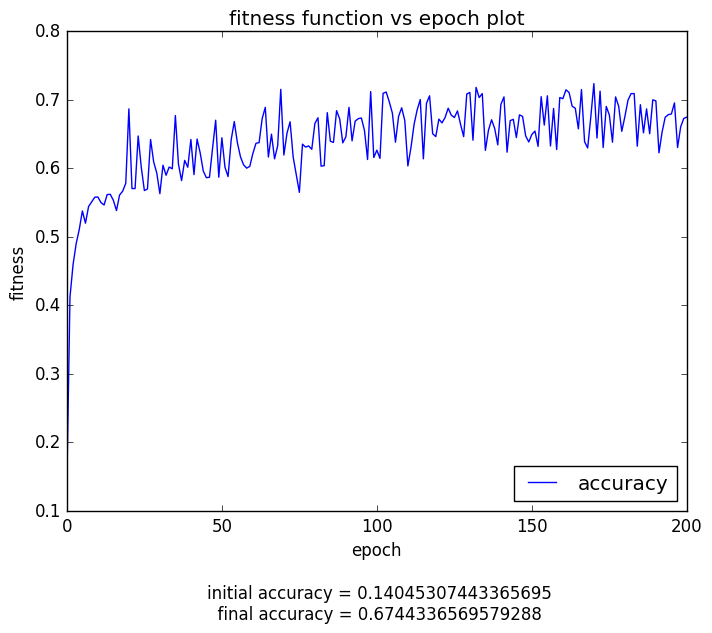
\includegraphics[scale=0.4]{img/20_acc_2.png}
\caption{Accuracy plot}
\end{figure}
\begin{figure}[H]
\centering
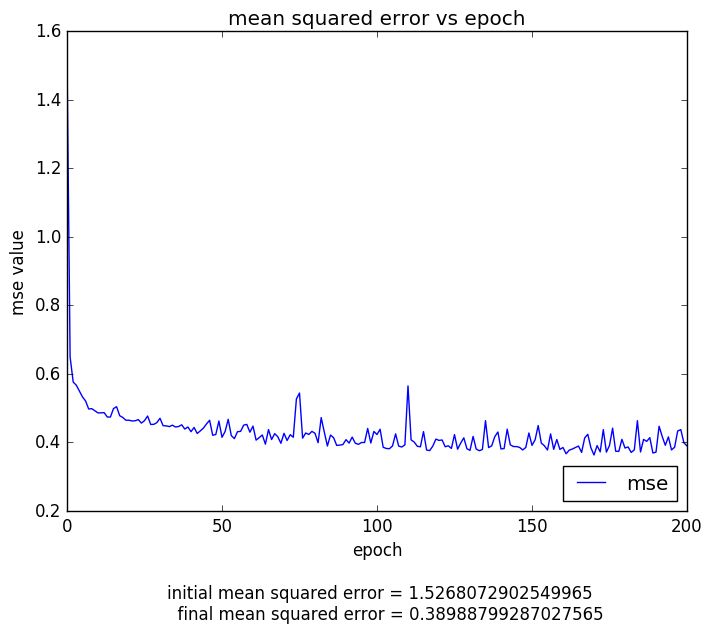
\includegraphics[scale=0.4]{img/20_mse_2.png}
\caption{MeanSquaredError plot}
\end{figure}

\subsection{50 features}
\subsubsection{1st configuration}
\begin{figure}[H]
\centering
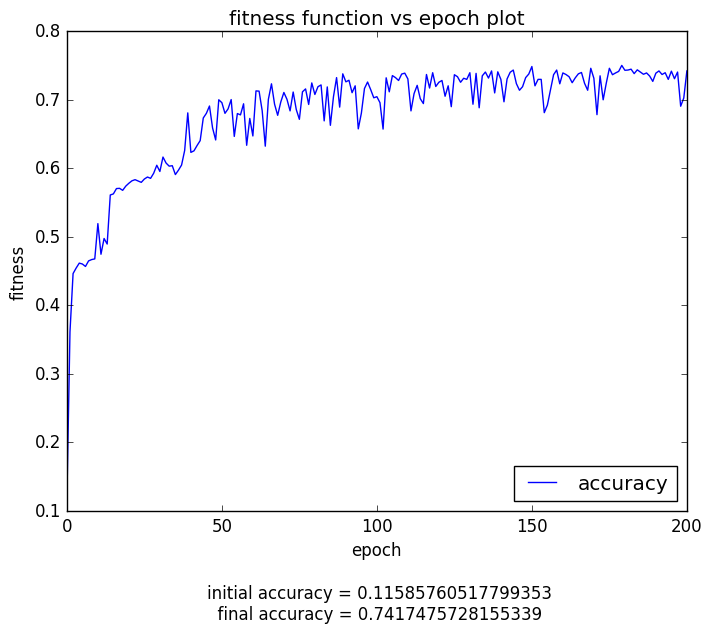
\includegraphics[scale=0.4]{img/50_acc.png}
\caption{Accuracy plot}
\end{figure}
\begin{figure}[H]
\centering
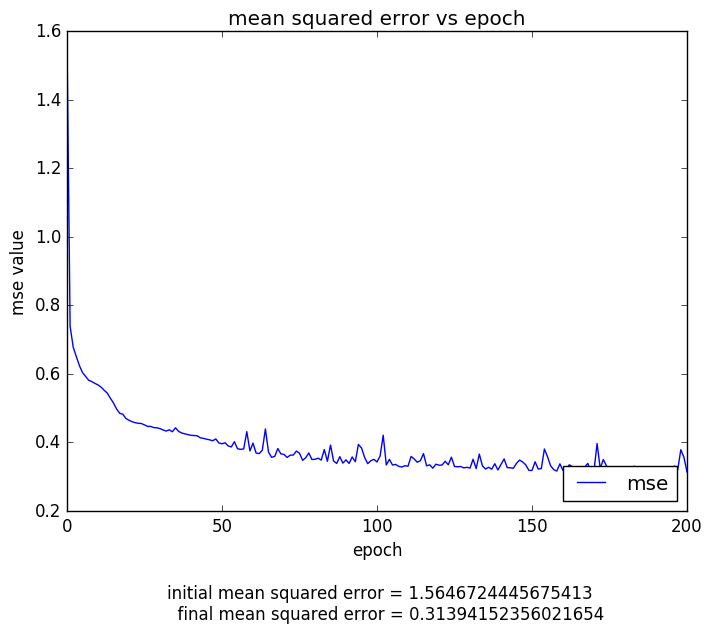
\includegraphics[scale=0.4]{img/50_mse.png}
\caption{MeanSquaredError plot}
\end{figure}

\subsubsection{2nd configuration}
\begin{figure}[H]
\centering
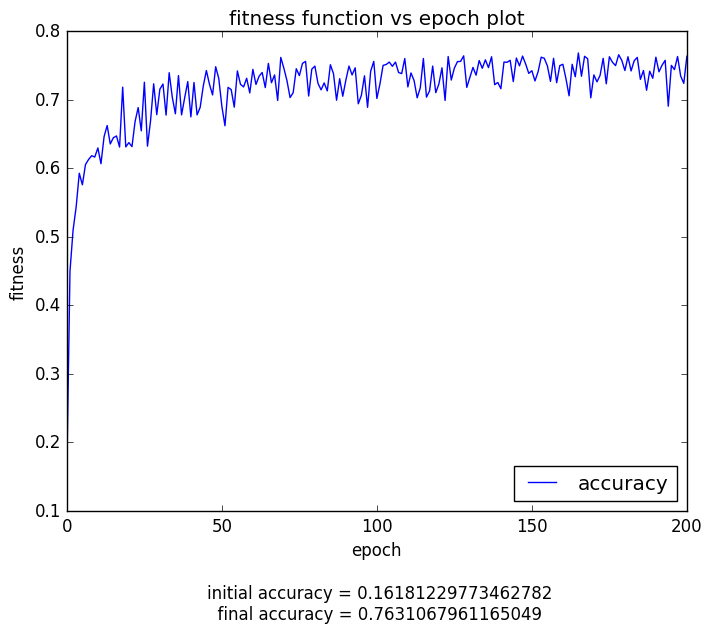
\includegraphics[scale=0.4]{img/50_acc_2.png}
\caption{Accuracy plot}
\end{figure}
\begin{figure}[H]
\centering
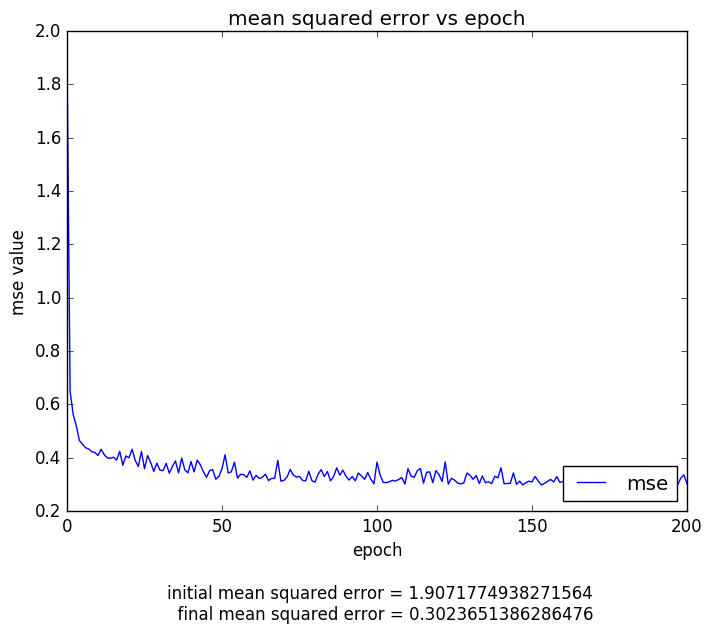
\includegraphics[scale=0.4]{img/50_mse_2.png}
\caption{MeanSquaredError plot}
\end{figure}

\subsection{561 features}
\subsubsection{1st configuration}
\begin{figure}[H]
\centering
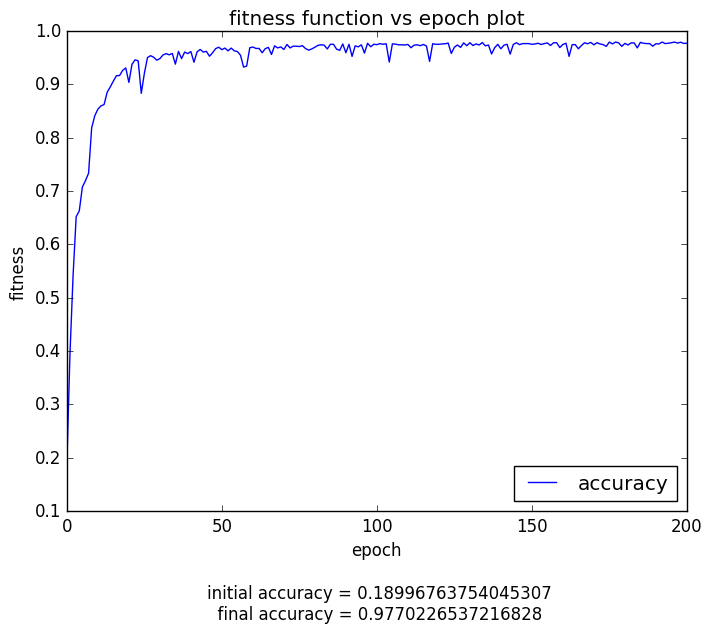
\includegraphics[scale=0.4]{img/all_acc.png}
\caption{Accuracy plot}
\end{figure}
\begin{figure}[H]
\centering
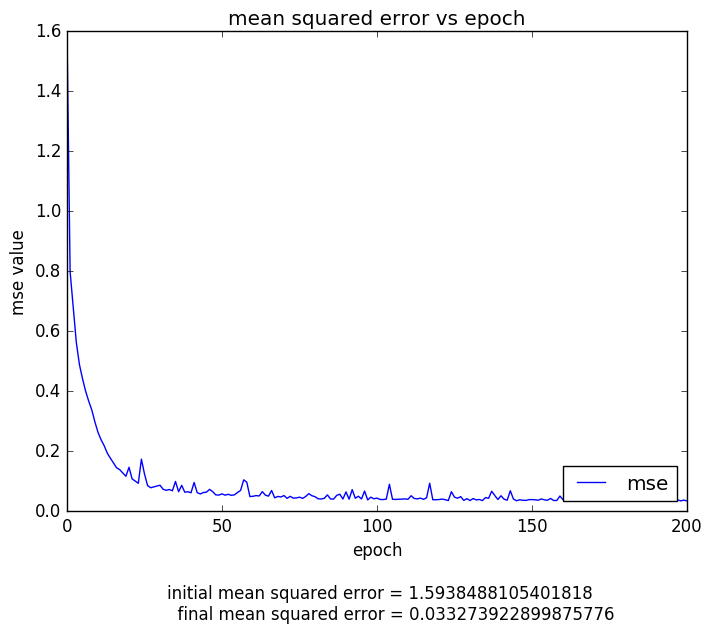
\includegraphics[scale=0.4]{img/all_mse.png}
\caption{MeanSquaredError plot}
\end{figure}

\subsubsection{2nd configuration}
\begin{figure}[H]
\centering
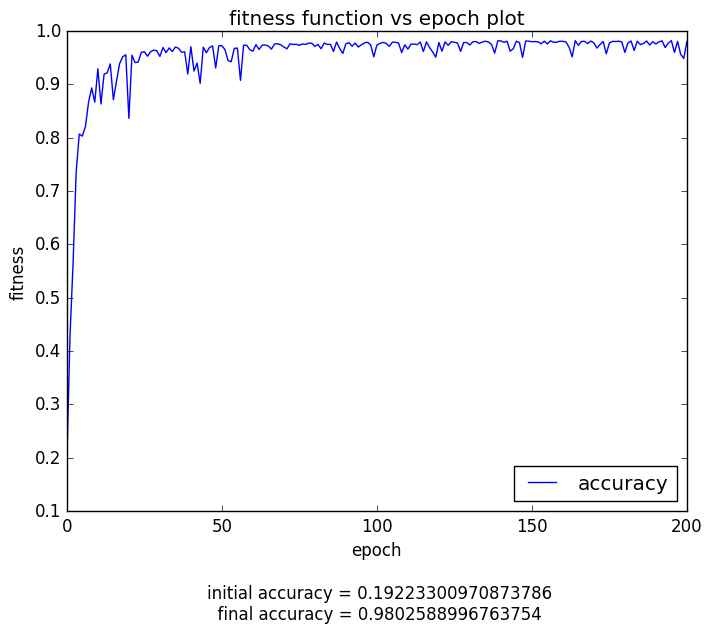
\includegraphics[scale=0.4]{img/all_acc_2.png}
\caption{Accuracy plot}
\end{figure}
\begin{figure}[H]
\centering
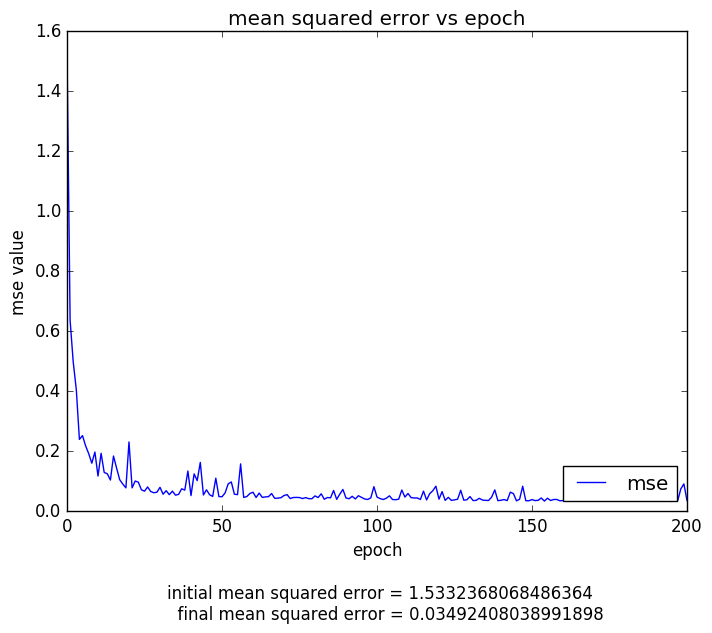
\includegraphics[scale=0.4]{img/all_mse_2.png}
\caption{MeanSquaredError plot}
\end{figure}

\subsection{8 and 561 features}
\begin{figure}[H]
\centering
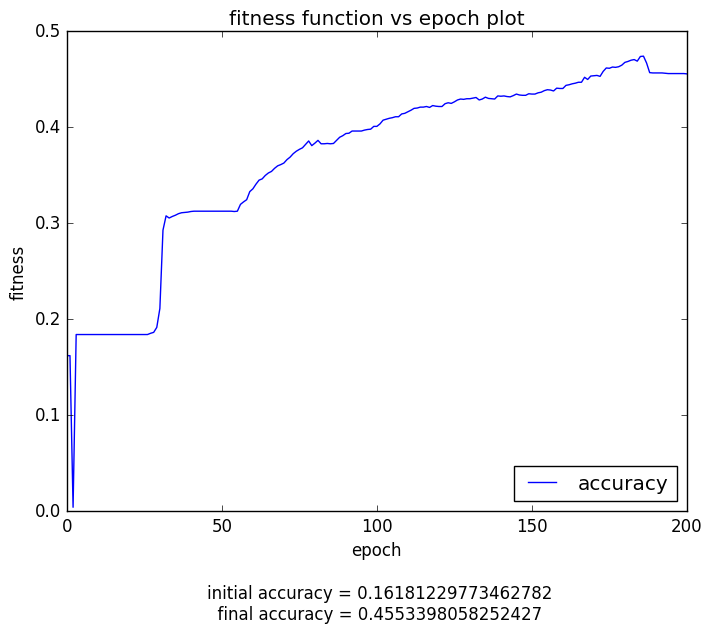
\includegraphics[scale=0.4]{img/8_3_acc.png}
\caption{Accuracy on 8 features plot}
\end{figure}
\begin{figure}[H]
\centering
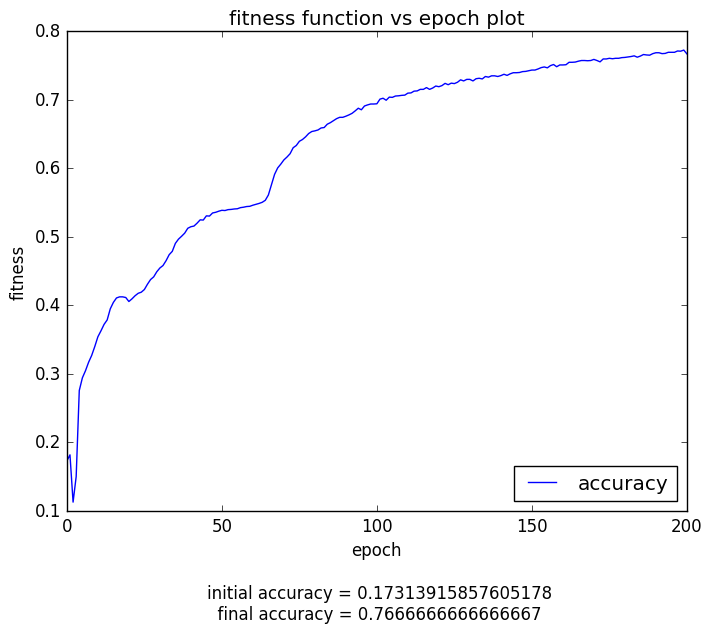
\includegraphics[scale=0.4]{img/all_3_acc.png}
\caption{Accuracy on all features plot}
\end{figure}

\subsection{Conclusion}

Due to fact that we performed experiments on different network structures and datasets build with wide variety of attibutes, we can conlude few remarks. Below we present our observations:
\begin{enumerate}
\item If the neural net is complex, it requires more epochs to gain satisfactionary accuracy. The backpropagation method requires more iterations to change synaptic weights in order to increase te accuracy and decrease overall mean squared error of the net.
\item The mean squared error is strictly related to overall accuracy. We can observe accuracy gains on mse drops.
\item Neural net with more complex structure can archieve a little bit better performance in comparison to the regular (not as complex) network.
\item High value of learning step provides dynamic mse growths causing accuracy drop. Big value of learning step causes net to update weights in conjunction with current instance, but weights change is so high that net forgets previous instances which were correctly classified.
\item Our experiment shows, that we do not increase accuracy when we decrease number of features in the dataset. The plots are similar in shape, but the accuracy is always worse than accuracy obtained when we trained net on the dataset with all features.
\item Time taken to fully train the net (iterate over all epochs) using dataset with all features is higher than training with only subset of features.
\end{enumerate}
 

\end{document}
\grid
